\documentclass[tikz,border=5pt]{standalone}
\usepackage{lmodern}
\renewcommand{\familydefault}{\sfdefault}
\usetikzlibrary{arrows.meta,calc,backgrounds}
% Training-recipe figures: match Ch 3's rlhf-basic.png / rlhf-complex.png.
% Latin Modern Sans, unfilled-looking boxes, gray open arrowheads, soft elbows.
% Requires \usetikzlibrary{arrows.meta,calc} and \usepackage{lmodern}.
% Compile with \def\figdark{1} for the site's slate dark theme.
\providecommand{\figdark}{0}
\ifnum\figdark=1
  \definecolor{recipebackground}{HTML}{1E293B}
  \definecolor{recipeborder}{HTML}{CBD5E1}
  \definecolor{recipetext}{HTML}{CBD5E1}
  \definecolor{recipearrow}{HTML}{94A3B8}
\else
  \definecolor{recipebackground}{HTML}{FFFFFF}
  \definecolor{recipeborder}{HTML}{262626}
  \definecolor{recipetext}{HTML}{333333}
  \definecolor{recipearrow}{HTML}{A6A6A6}
\fi

\tikzset{
  recipe model/.style={
    rectangle, rounded corners=2pt,
    draw=recipeborder, fill=recipebackground, text=recipetext,
    line width=1.05pt,
    minimum width=2.8cm, minimum height=0.95cm,
    inner xsep=7pt, inner ysep=5pt,
    font=\fontsize{14}{17}\selectfont, align=center
  },
  recipe line/.style={
    draw=recipearrow, line width=1.4pt,
    line cap=round, line join=round, rounded corners=7pt
  },
  recipe arrow/.style={
    recipe line,
    -{Straight Barb[length=2.7mm,width=4.2mm]}, shorten >=5pt
  },
  recipe label/.style={
    text=recipetext, font=\fontsize{10}{13}\selectfont,
    align=center, inner sep=2pt
  },
  recipe operation/.style={recipe label, font=\fontsize{10}{13}\selectfont\itshape},
  recipe edge operation/.style={recipe operation, anchor=south, yshift=5pt},
  recipe example/.style={
    recipe label, font=\fontsize{8.5}{10}\selectfont,
    anchor=north, inner sep=0pt, yshift=-3pt
  }
}


% Generic specialist-training pattern, inspired by MiMo-V2-Flash and
% Nemotron 3 Ultra, not a literal reconstruction of either full recipe.
% Every illustrated expert receives its own SFT and RL after shared SFT.
% Teacher indices indicate domains; N is arbitrary, not a reported count.
% One illustrative domain example labels each teacher's SFT/RL row.
% MOPD transfers teacher distributions on student rollouts, not model weights.
% Sources and deliberate simplifications: see this directory's README.md.
\begin{document}
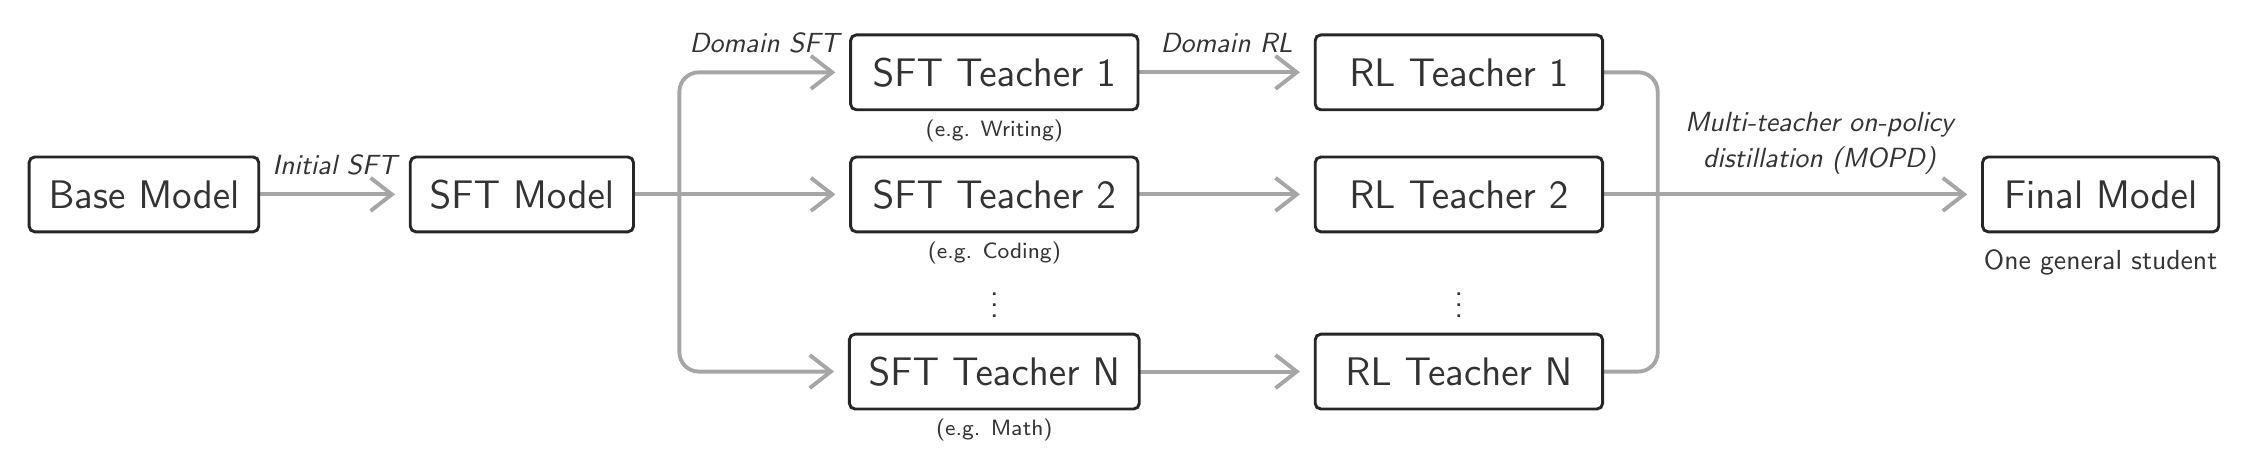
\begin{tikzpicture}
  \node[recipe model] (base) at (0,0) {Base Model};
  \node[recipe model] (sft) at (4.8,0) {SFT Model};

  \node[recipe model,minimum width=3.65cm] (sftone) at (10.8,1.55) {SFT Teacher 1};
  \node[recipe model,minimum width=3.65cm] (sfttwo) at (10.8,0) {SFT Teacher 2};
  \node[recipe model,minimum width=3.65cm] (sftn) at (10.8,-2.25) {SFT Teacher N};
  \node[recipe model,minimum width=3.65cm] (rlone) at (16.7,1.55) {RL Teacher 1};
  \node[recipe model,minimum width=3.65cm] (rltwo) at (16.7,0) {RL Teacher 2};
  \node[recipe model,minimum width=3.65cm] (rln) at (16.7,-2.25) {RL Teacher N};
  \node[recipe label,font=\large] at (10.8,-1.3) {$\vdots$};
  \node[recipe label,font=\large] at (16.7,-1.3) {$\vdots$};

  \node[recipe example] at (sftone.south) {(e.g. Writing)};
  \node[recipe example] at (sfttwo.south) {(e.g. Coding)};
  \node[recipe example] at (sftn.south) {(e.g. Math)};

  \node[recipe model,minimum width=3cm] (final) at (24.85,0) {Final Model};

  \coordinate (split) at (6.8,0);
  \coordinate (branchtop) at (split |- sftone.west);
  \coordinate (merge) at (19.225,0);

  % Draw connections behind the opaque boxes and their outlines.
  \begin{scope}[on background layer]
    \draw[recipe arrow] (base.east) -- (sft.west);

    % A single shared SFT checkpoint seeds the separate domain specialists.
    \draw[recipe line] (sft.east) -- (split);
    \draw[recipe arrow] (split) |- (sftone.west);
    \draw[recipe arrow] (split) -- (sfttwo.west);
    \draw[recipe arrow] (split) |- (sftn.west);

    \draw[recipe arrow] (sftone.east) -- (rlone.west);
    \draw[recipe arrow] (sfttwo.east) -- (rltwo.west);
    \draw[recipe arrow] (sftn.east) -- (rln.west);

    % The branches converge through distillation into one general student.
    \draw[recipe line] (rlone.east) -| (merge);
    \draw[recipe line] (rltwo.east) -- (merge);
    \draw[recipe line] (rln.east) -| (merge);
    \draw[recipe arrow] (merge) -- (final.west);
  \end{scope}

  % Each operation sits just above the line it describes.
  \node[recipe edge operation] at ($(base.east)!0.5!(sft.west)$) {Initial SFT};
  \node[recipe edge operation] at ($(branchtop)!0.5!(sftone.west)$) {Domain SFT};
  \node[recipe edge operation] at ($(sftone.east)!0.5!(rlone.west)$) {Domain RL};
  \node[recipe edge operation] at ($(merge)!0.5!(final.west)$) {Multi-teacher on-policy\\distillation (MOPD)};
  \node[recipe label,anchor=north,yshift=-4pt] at (final.south) {One general student};
\end{tikzpicture}
\end{document}
